\documentclass[11pt,a4paper]{article}

% Packages
\usepackage[margin=2.2cm]{geometry}
\usepackage{graphicx}
\usepackage{xcolor}
\usepackage{hyperref}
\usepackage{array}
\usepackage{booktabs}
\usepackage{tabularx}
\usepackage{fancyhdr}
\usepackage{lastpage}
\usepackage{fontspec}
\usepackage{setspace}
\usepackage{tikz}
\usepackage{enumitem}
\usepackage{multicol}
\usepackage{tcolorbox}
\usepackage{float}
\usepackage{amssymb}
\usepackage{amsmath}
\usepackage{listings}
\usepackage{fontawesome5}

\usetikzlibrary{shapes.geometric, arrows.meta, positioning, fit, backgrounds, calc, decorations.pathreplacing}
\tcbuselibrary{skins, breakable}

% Wispy Colors
\definecolor{wispyblack}{HTML}{000000}
\definecolor{wispycyan}{HTML}{00DDFF}
\definecolor{wispymagenta}{HTML}{FF00E9}
\definecolor{wispyorange}{HTML}{FF7000}
\definecolor{wispyyellow}{HTML}{FFF700}
\definecolor{wispylight}{HTML}{F0FDFF}
\definecolor{wispymaglight}{HTML}{FFF0FE}
\definecolor{wispyorangelight}{HTML}{FFF5F0}
\definecolor{wispyyellowlight}{HTML}{FFFEF0}
\definecolor{sectionbg}{HTML}{FAFAFA}
\definecolor{codebg}{HTML}{1E1E1E}
\definecolor{codetext}{HTML}{D4D4D4}

% Fonts
\setmainfont{Calibri}
\setmonofont{Consolas}

% Custom column types
\newcolumntype{L}[1]{>{\raggedright\arraybackslash}p{#1}}
\newcolumntype{C}[1]{>{\centering\arraybackslash}p{#1}}
\newcolumntype{R}[1]{>{\raggedleft\arraybackslash}p{#1}}
\newcolumntype{Y}{>{\raggedright\arraybackslash}X}

% Code listing style
\lstdefinestyle{wispycode}{
  backgroundcolor=\color{codebg},
  basicstyle=\ttfamily\small\color{codetext},
  breaklines=true,
  captionpos=b,
  keepspaces=true,
  showspaces=false,
  showstringspaces=false,
  frame=none,
  xleftmargin=4mm,
  xrightmargin=4mm,
  aboveskip=3mm,
  belowskip=3mm
}
\lstset{style=wispycode}

% Custom boxes
\newtcolorbox{wispybox}[1][]{
  enhanced, colback=wispylight, colframe=wispycyan,
  fonttitle=\bfseries\normalsize\color{wispyblack},
  coltitle=wispyblack, colbacktitle=wispycyan!30,
  attach boxed title to top left={yshift=-2mm, xshift=5mm},
  boxed title style={sharp corners, boxrule=0pt},
  sharp corners, boxrule=1pt,
  top=4mm, bottom=4mm, left=4mm, right=4mm,
  before skip=6mm, after skip=6mm, #1
}

\newtcolorbox{problembox}[1][]{
  enhanced, colback=wispymaglight, colframe=wispymagenta,
  fonttitle=\bfseries\normalsize\color{wispyblack},
  coltitle=wispyblack, colbacktitle=wispymagenta!30,
  attach boxed title to top left={yshift=-2mm, xshift=5mm},
  boxed title style={sharp corners, boxrule=0pt},
  sharp corners, boxrule=1pt,
  top=4mm, bottom=4mm, left=4mm, right=4mm,
  before skip=6mm, after skip=6mm, #1
}

\newtcolorbox{solutionbox}[1][]{
  enhanced, colback=wispyorangelight, colframe=wispyorange,
  fonttitle=\bfseries\normalsize\color{wispyblack},
  coltitle=wispyblack, colbacktitle=wispyorange!30,
  attach boxed title to top left={yshift=-2mm, xshift=5mm},
  boxed title style={sharp corners, boxrule=0pt},
  sharp corners, boxrule=1pt,
  top=4mm, bottom=4mm, left=4mm, right=4mm,
  before skip=6mm, after skip=6mm, #1
}

\newtcolorbox{hackathonbox}[1][]{
  enhanced, colback=wispyyellowlight, colframe=wispyyellow!80!black,
  fonttitle=\bfseries\normalsize\color{wispyblack},
  coltitle=wispyblack, colbacktitle=wispyyellow,
  attach boxed title to top left={yshift=-2mm, xshift=5mm},
  boxed title style={sharp corners, boxrule=0pt},
  sharp corners, boxrule=1pt,
  top=4mm, bottom=4mm, left=4mm, right=4mm,
  before skip=6mm, after skip=6mm, #1
}

\newtcolorbox{codebox}[1][]{
  enhanced, colback=codebg, colframe=gray!50,
  fonttitle=\bfseries\ttfamily\small\color{white},
  sharp corners, boxrule=0.5pt,
  left=3mm, right=3mm, top=3mm, bottom=3mm, #1
}

\renewcommand{\arraystretch}{1.3}

% Header and Footer
\pagestyle{fancy}
\fancyhf{}
\fancyhead[L]{\small\color{wispyblack}Wispy Console --- Technical Whitepaper v1.0}
\fancyhead[R]{\small\color{wispyblack}hausorlabs.tech}
\fancyfoot[C]{\small\color{wispyblack}Page \thepage\ of \pageref{LastPage}}
\renewcommand{\headrulewidth}{0.4pt}
\renewcommand{\footrulewidth}{0.4pt}

\hypersetup{
  colorlinks=true,
  linkcolor=wispycyan!80!black,
  urlcolor=wispymagenta!80!black,
  citecolor=wispyorange
}

\begin{document}

% ============================================================
% TITLE PAGE
% ============================================================
\thispagestyle{empty}

\begin{center}

\vspace*{1.5cm}

% Logo accent bar

\begin{tikzpicture}
  \fill[wispycyan] (0,0) rectangle (4,0.15);
  \fill[wispymagenta] (4.2,0) rectangle (8.2,0.15);
  \fill[wispyorange] (8.4,0) rectangle (12.4,0.15);
  \fill[wispyyellow] (12.6,0) rectangle (16.6,0.15);
\end{tikzpicture}

\vspace{1.2cm}

{\fontsize{42}{50}\selectfont\bfseries\color{wispyblack} WISPY CONSOLE}

\vspace{0.4cm}

{\Large\color{gray!70!black} AI Agent Control Center for Logitech MX Creative Console}

\vspace{1.8cm}

% Four Pillars TikZ Diagram
\begin{tikzpicture}[
  pillar/.style={
    draw=#1, fill=#1!8, line width=1.5pt,
    minimum width=3.4cm, minimum height=4.2cm,
    rounded corners=3pt, align=center, font=\small
  },
  pillarlabel/.style={
    font=\bfseries\normalsize, color=wispyblack
  },
  pillaricon/.style={
    font=\fontsize{28}{32}\selectfont, color=#1
  }
]

% Pillar 1: LCD Buttons
\node[pillar=wispycyan] (p1) at (0,0) {};
\node[pillaricon=wispycyan] at (0, 0.8) {\faThLarge};
\node[pillarlabel] at (0, -0.1) {9 LCD Buttons};
\node[font=\scriptsize, text width=2.8cm, align=center, color=gray!70!black] at (0, -0.9) {Dynamic actions\\Real-time status\\15 pages};

% Pillar 2: Thinking Dial
\node[pillar=wispymagenta] (p2) at (4.2,0) {};
\node[pillaricon=wispymagenta] at (4.2, 0.8) {\faSlidersH};
\node[pillarlabel] at (4.2, -0.1) {Thinking Dial};
\node[font=\scriptsize, text width=2.8cm, align=center, color=gray!70!black] at (4.2, -0.9) {Graduated control\\Flash to Marathon\\Press to reset};

% Pillar 3: Actions Ring
\node[pillar=wispyorange] (p3) at (8.4,0) {};
\node[pillaricon=wispyorange] at (8.4, 0.8) {\faCircleNotch};
\node[pillarlabel] at (8.4, -0.1) {Actions Ring};
\node[font=\scriptsize, text width=2.8cm, align=center, color=gray!70!black] at (8.4, -0.9) {Context-aware\\Auto-switching\\MX Master 4};

% Pillar 4: Haptic Feedback
\node[pillar=wispyyellow!80!black] (p4) at (12.6,0) {};
\node[pillaricon=wispyyellow!60!black] at (12.6, 0.8) {\faWaveSquare};
\node[pillarlabel] at (12.6, -0.1) {Haptic Feedback};
\node[font=\scriptsize, text width=2.8cm, align=center, color=gray!70!black] at (12.6, -0.9) {State awareness\\6 patterns\\Feel the agent};

% Connecting line beneath
\draw[wispycyan, line width=1pt, dashed] (p1.south) -- ++(0,-0.6) -| (p4.south);

\end{tikzpicture}

\vspace{1.8cm}


\begin{tikzpicture}
  \node[draw=wispyyellow!80!black, fill=wispyyellowlight, rounded corners=5pt, inner sep=10pt, line width=1pt] {
    \Large\bfseries\color{wispyblack} DevStudio 2026 by Logitech
  };
\end{tikzpicture}

\vspace{1.2cm}

{\large Version 1.0 -- February 2026}

\vspace{0.8cm}

{\large\bfseries Brian Mwai \& Joy Chepkoech Lang'at}\\[0.3cm]
{\large Hausor Labs}

\vspace{1.5cm}

% Bottom accent bar

\begin{tikzpicture}
  \fill[wispyyellow] (0,0) rectangle (4,0.15);
  \fill[wispyorange] (4.2,0) rectangle (8.2,0.15);
  \fill[wispymagenta] (8.4,0) rectangle (12.4,0.15);
  \fill[wispycyan] (12.6,0) rectangle (16.6,0.15);
\end{tikzpicture}

\end{center}

\newpage

% ============================================================
% TABLE OF CONTENTS
% ============================================================
\tableofcontents

\newpage

% ============================================================
% SECTION 1: EXECUTIVE SUMMARY
% ============================================================
\section{Executive Summary}

\begin{wispybox}[title={\faRocket~Wispy Console: The Physical Layer for AI Agents}, breakable]

\textbf{Wispy Console} is a Logitech Actions SDK plugin that transforms the MX Creative Console into a universal AI agent control center. It bridges the gap between software-only AI workflows and the tactile, spatial intelligence of physical hardware.

\vspace{3mm}

The plugin provides four core capabilities:

\begin{itemize}[leftmargin=5mm, itemsep=2mm]
  \item \textbf{9 LCD Buttons} for agent actions, each displaying real-time status with dynamic icons, organized across up to 15 pages for a total of 135 possible actions.
  \item \textbf{A Precision Dial} for controlling thinking depth, offering graduated autonomy from quick Flash responses to deep Marathon reasoning sessions.
  \item \textbf{Actions Ring} on the MX Master 4 for context-aware agent switching, automatically mapping the active application to the appropriate AI agent.
  \item \textbf{Haptic Feedback} for state awareness, allowing developers to feel the agent's status (success, error, state changes) through six distinct vibration patterns.
\end{itemize}

\vspace{3mm}

Wispy Console connects to any AI agent through a universal adapter interface, making it hardware-agnostic on the agent side and agent-agnostic on the hardware side. The reference implementation targets \textbf{Wispy v1.4.1} (published on npm as \texttt{wispy-ai}), powered by \textbf{Google Gemini 2.5 Pro}, with adapters planned for Claude Code, Aider, OpenClaw, and any REST-compatible agent.

\vspace{3mm}

This is the \textbf{first AI plugin designed for the Logitech Marketplace}, establishing a new category of physical AI interaction that no software-only solution can replicate.

\end{wispybox}

\subsection{Key Metrics}

\begin{center}
\begin{tabularx}{\textwidth}{C{4cm} Y}
\toprule
\textbf{Metric} & \textbf{Value} \\
\midrule
Target Hardware & Logitech MX Creative Console + MX Master 4 \\
SDK & Logitech Actions SDK (TypeScript) \\
Agent Framework & Wispy v1.4.1 (\texttt{wispy-ai} on npm) \\
AI Engine & Google Gemini 2.5 Pro \\
Total Actions & Up to 135 (9 buttons $\times$ 15 pages) \\
Thinking Levels & 100 (continuous dial, 4 named zones) \\
Haptic Patterns & 6 distinct feedback types \\
Supported Agents & 2 native, 3 planned, unlimited via REST adapter \\
\bottomrule
\end{tabularx}
\end{center}

\newpage

% ============================================================
% SECTION 2: THE PROBLEM
% ============================================================
\section{The Problem}

AI coding agents have reached extraordinary capability, yet the developer experience of \textit{using} them remains fundamentally broken. Five interconnected problems create a crisis of productivity, trust, and accessibility that no software-only solution has resolved.

\subsection{Permission Fatigue}

\begin{problembox}[title={\faExclamationTriangle~The Approval Bottleneck}, breakable]

Every modern AI coding agent requires explicit human approval for tool calls, file modifications, and shell commands. In practice, this means developers tap ``approve'' every 10--15 seconds during active agent sessions.

\vspace{3mm}

The scale of this problem is documented extensively in open-source issue trackers:

\begin{itemize}[leftmargin=5mm, itemsep=2mm]
  \item \textbf{GitHub Issue \#11380} (30+ upvotes): Developers report that constant approval prompts make agents nearly unusable for sustained work sessions.
  \item \textbf{GitHub Issue \#2560}: Feature requests for bulk approval, auto-approval, and trust levels have accumulated hundreds of comments.
\end{itemize}

\vspace{3mm}

\textit{``I spend more time clicking `approve' than I do reviewing what the agent actually did.''} \\
\hfill --- @cmwalton, GitHub \#11380

\vspace{3mm}

\textit{``The approval flow is the single biggest bottleneck. The agent can think in 2 seconds but waits 30 seconds for me to context-switch back and click a button.''} \\
\hfill --- @cruftyoldsysadmin, GitHub \#2560

\vspace{3mm}

The core issue is not that approvals exist; they are essential for safety. The problem is that the \textit{interface} for approvals is a full-screen context switch that demands the developer's complete visual attention, breaking flow state every time.

\end{problembox}

\subsection{The YOLO Trap}

\begin{problembox}[title={\faBomb~Binary Choice: Babysit or Gamble}, breakable]

Faced with permission fatigue, developers are presented with exactly two options: supervise every action manually, or enable ``YOLO mode'' (auto-approve everything) and hope nothing goes wrong.

\vspace{3mm}

There is no middle ground. No graduated trust. No way to say \textit{``approve file reads automatically, but ask me before shell commands.''} The result is a binary gamble.

\vspace{3mm}

\textit{``YOLO mode is like giving your intern root access and going to lunch. You'll probably be fine. Probably.''} \\
\hfill --- @forrestthewoods, Hacker News

\vspace{3mm}

The consequences of getting this wrong are not hypothetical. \textbf{GitHub Issue \#12637} documents a case where an agent running in YOLO mode executed \texttt{rm -rf \textasciitilde/}, deleting the user's entire home directory. The developer had enabled auto-approve to avoid permission fatigue during a routine refactoring session.

\vspace{3mm}

This incident crystallizes the fundamental design failure: the only escape from permission fatigue is a mode that removes all safety guarantees. Developers need a continuous spectrum of control, not a binary switch.

\end{problembox}

\subsection{Context Switching}

\begin{problembox}[title={\faBrain~The 15-Minute Recovery}, breakable]

AI agents operate in terminal windows, chat interfaces, and IDE sidebars. Monitoring their progress requires switching away from productive work to check status, review output, and respond to prompts.

\vspace{3mm}

Research consistently shows that context switches cost 15--30 minutes of productive recovery time:

\vspace{3mm}

\textit{``Every time I switch to the agent's terminal to check progress, I lose my train of thought on the actual code I was reviewing. It's a 15-minute recovery each time.''} \\
\hfill --- @PetahNZ, Hacker News

\vspace{3mm}

\textit{``The irony of AI assistants is that they create more context switches than they eliminate. I'm constantly alt-tabbing to babysit something that's supposed to be autonomous.''} \\
\hfill --- @ak217, Hacker News

\vspace{3mm}

The problem compounds with multiple agents. \textbf{GitHub Issue \#15898} documents a developer (@midlifedad) managing 12 simultaneous AI instances across different projects, each requiring periodic attention, approval, and status monitoring. The cognitive overhead of tracking 12 independent state machines through terminal windows alone is unsustainable.

\end{problembox}

\subsection{The Trust Crisis}

\begin{problembox}[title={\faShieldAlt~Declining Confidence in AI Output}, breakable]

Even when agents produce output, developers increasingly distrust it. The \textbf{Stack Overflow 2025 Developer Survey} reveals a stark picture:

\vspace{3mm}

\begin{center}
\begin{tabular}{L{9cm} R{4cm}}
\toprule
\textbf{Finding} & \textbf{Statistic} \\
\midrule
Developers who spend more time \textit{correcting} AI output than it saved & \textbf{66\%} \\
Cite ``almost right'' code as the \#1 frustration & \textbf{45\%} \\
Trust in AI-generated code (down from 40\%) & \textbf{29\%} \\
Prefer human-written code for production & \textbf{75\%} \\
\bottomrule
\end{tabular}
\end{center}

\vspace{3mm}

The ``almost right'' problem is particularly insidious. Code that looks correct, passes a cursory review, but contains subtle logical errors is worse than obviously wrong code because it bypasses human scrutiny. Without a mechanism to control the \textit{depth} of AI reasoning, developers cannot trade speed for correctness when the stakes demand it.

\end{problembox}

\subsection{The Accessibility Gap}

\begin{problembox}[title={\faUniversalAccess~AI Tools Exclude Disabled Developers}, breakable]

The \textbf{CHI 2025 Conference on Human-Computer Interaction} published research showing that AI coding tools \textit{``exacerbated existing accessibility barriers''} rather than reducing them.

\vspace{3mm}

Key findings include:

\begin{itemize}[leftmargin=5mm, itemsep=2mm]
  \item \textbf{Screen readers cannot navigate} the rapid, streaming output of AI agents. Text arrives faster than assistive technology can process it, creating an incomprehensible experience.
  \item \textbf{RSI sufferers cannot sustain} the repetitive keyboard and mouse inputs required by permission approval workflows. Dozens of approvals per session, each requiring precise targeting of small UI elements, causes physical pain.
  \item \textbf{Visual impairments} make it impossible to scan long agent outputs for errors. The primary interface for all major AI agents is dense, scrolling text.
  \item \textbf{Motor disabilities} make rapid approval workflows inaccessible. The time pressure of agents waiting for approval combines with small click targets to exclude developers with limited motor control.
\end{itemize}

\vspace{3mm}

Physical hardware with large buttons, tactile feedback, and non-visual state communication is not merely a convenience improvement for these users; it is an accessibility requirement.

\end{problembox}

\newpage

% ============================================================
% SECTION 3: THE SOLUTION
% ============================================================
\section{The Solution}

Wispy Console addresses each of the five problems through purpose-built hardware interactions that operate in parallel with the developer's primary workflow. No context switching. No binary choices. No accessibility barriers.

\subsection{The Keypad: 9 LCD Buttons}

\begin{solutionbox}[title={\faThLarge~Dynamic Action Grid}, breakable]

The MX Creative Console features 9 programmable LCD buttons arranged in a 3$\times$3 grid. Each button displays a dynamic icon and label that updates in real time based on agent state. The console supports 15 pages of button configurations, providing up to 135 distinct actions.

\vspace{3mm}

\textbf{Default Button Layout (Page 1):}

\vspace{3mm}

\begin{center}
\begin{tabular}{|C{3.8cm}|C{3.8cm}|C{3.8cm}|}
\hline
\rowcolor{wispylight}
\textbf{\faCode~Code} & \textbf{\faSearch~Research} & \textbf{\faRocket~Deploy} \\
\small Send coding task & \small Web research query & \small Run deployment \\
\hline
\rowcolor{wispylight}
\textbf{\faCheck~Approve} & \textbf{\faTimes~Reject} & \textbf{\faMicrophone~Voice} \\
\small Approve pending action & \small Reject with feedback & \small Voice command input \\
\hline
\rowcolor{wispylight}
\textbf{\faChartBar~Status} & \textbf{\faBolt~Quick} & \textbf{\faExchangeAlt~Mode} \\
\small Agent status overview & \small Quick action shortcut & \small Switch agent mode \\
\hline
\end{tabular}
\end{center}

\vspace{3mm}

Each LCD dynamically updates to reflect context. When an agent requests approval, the \textbf{Approve} button pulses green and displays the pending action summary. When an error occurs, the \textbf{Status} button turns red and shows the error type. This eliminates the need to switch to a terminal to understand agent state.

\vspace{3mm}

\textbf{Page Organization (15 Pages):}

\begin{itemize}[leftmargin=5mm, itemsep=1mm]
  \item \textbf{Pages 1--3}: Core actions (code, research, deploy, approve/reject, voice, status)
  \item \textbf{Pages 4--6}: Tool-specific actions (file operations, git, terminal, browser)
  \item \textbf{Pages 7--9}: Agent-specific actions (Wispy tools, OpenClaw commands, custom)
  \item \textbf{Pages 10--12}: Project profiles (frontend, backend, DevOps, data)
  \item \textbf{Pages 13--15}: User-customizable pages for personal workflows
\end{itemize}

\vspace{3mm}

This solves \textbf{permission fatigue} by providing a dedicated physical button for approve/reject that requires zero context switching. The developer's eyes never leave their primary monitor. A single thumb press on a tactile button replaces the full interrupt cycle of alt-tab, locate prompt, click approve, alt-tab back.

\end{solutionbox}

\subsection{Thinking Depth Dial}

\begin{solutionbox}[title={\faSlidersH~Graduated Autonomy Control}, breakable]

The MX Creative Console's precision dial maps to a continuous thinking depth scale from 0 to 100. Four named zones provide intuitive reference points, while the continuous range allows fine-grained control.

\vspace{3mm}

\begin{center}
\begin{tabular}{C{2.5cm} C{2cm} L{8cm}}
\toprule
\textbf{Zone} & \textbf{Range} & \textbf{Behavior} \\
\midrule
\rowcolor{wispylight}
\textbf{Flash} & 0--20 & Quick responses, minimal reasoning. Auto-approves safe operations (file reads, searches). Best for rapid iteration and exploration. \\
\textbf{Standard} & 21--50 & Balanced reasoning with selective approval. Approves known-safe patterns, prompts for modifications and shell commands. Default mode. \\
\rowcolor{wispylight}
\textbf{Deep Think} & 51--80 & Extended reasoning with careful review. Requires approval for all file modifications. Uses chain-of-thought prompting for complex tasks. \\
\textbf{Marathon} & 81--100 & Maximum reasoning depth. Full approval required for everything. Activates Wispy's Marathon mode for multi-step planning and execution. Red haptic zone. \\
\bottomrule
\end{tabular}
\end{center}

\vspace{3mm}

\textbf{Press to Reset}: Pressing the dial resets thinking depth to Standard (35), providing a quick escape from any zone.

\vspace{3mm}

This is the \textbf{middle ground between YOLO and babysitting}. Instead of a binary on/off for auto-approval, the dial provides a continuous spectrum. Turning it left toward Flash gives more autonomy for routine tasks. Turning it right toward Marathon engages maximum caution for critical operations. The physical position of the dial is always visible and tactile, providing ambient awareness of the current trust level without any screen interaction.

\vspace{3mm}

This directly addresses the \textbf{YOLO trap}. The dial's physical position in the Marathon zone (81--100) creates a deliberate ``danger zone'' with distinct haptic resistance, making it impossible to accidentally leave the agent in high-autonomy mode. The graduated control means developers can find their personal comfort level rather than choosing between two extremes.

\end{solutionbox}

\subsection{Actions Ring: MX Master 4}

\begin{solutionbox}[title={\faCircleNotch~Context-Aware Agent Switching}, breakable]

The MX Master 4's Actions Ring (horizontal scroll wheel) provides context-aware agent switching. As the developer moves between applications, the ring automatically maps the active window to the most appropriate AI agent.

\vspace{3mm}

\begin{center}
\begin{tabular}{C{3cm} C{3cm} L{6.5cm}}
\toprule
\textbf{Active App} & \textbf{Agent} & \textbf{Behavior} \\
\midrule
\rowcolor{wispylight}
VS Code & Coder Agent & Code generation, refactoring, debugging, testing \\
Chrome / Browser & Research Agent & Web research, documentation lookup, API exploration \\
\rowcolor{wispylight}
Terminal & DevOps Agent & Deployment, infrastructure, shell commands, CI/CD \\
Figma & Analyst Agent & Design analysis, component generation, style extraction \\
\bottomrule
\end{tabular}
\end{center}

\vspace{3mm}

The Actions Ring also supports manual override: scrolling the ring cycles through available agents regardless of the active application. This provides both automatic convenience and manual control.

\vspace{3mm}

This solves the \textbf{context switching} problem for multi-agent workflows. Instead of managing 12 terminal windows, the developer's physical environment tracks which agent is active. The ring's position is a spatial memory aid, similar to how a musician's hand position on an instrument provides subconscious state awareness.

\end{solutionbox}

\subsection{Haptic Feedback}

\begin{solutionbox}[title={\faWaveSquare~Feel the Agent's State}, breakable]

The MX Creative Console's haptic motor provides six distinct vibration patterns that communicate agent state through touch. This enables developers to monitor agent progress without looking at any screen.

\vspace{3mm}

\begin{center}
\begin{tabular}{L{3.8cm} L{3cm} L{5.5cm}}
\toprule
\textbf{Pattern} & \textbf{SDK Name} & \textbf{Meaning} \\
\midrule
\rowcolor{wispylight}
Short double pulse & \texttt{happy\_alert} & Agent completed a task successfully \\
Long sustained buzz & \texttt{completed} & Multi-step operation finished \\
\rowcolor{wispylight}
Sharp triple pulse & \texttt{angry\_alert} & Error or failure occurred \\
Single strong tap & \texttt{sharp\_state\_change} & Agent switched state (idle to active) \\
\rowcolor{wispylight}
Gentle wave & \texttt{wave} & Agent is thinking (continuous) \\
Two firm taps & \texttt{knock} & Agent needs attention (approval pending) \\
\bottomrule
\end{tabular}
\end{center}

\vspace{3mm}

\textit{Feel the agent's state in your hand.} When the console vibrates with a ``knock'' pattern, the developer knows approval is needed without checking any screen. When a ``happy\_alert'' pulses, the task succeeded. When ``angry\_alert'' fires, something went wrong.

\vspace{3mm}

This is the most significant \textbf{accessibility} improvement. Haptic feedback communicates state through touch, serving developers with visual impairments, those using screen readers, and anyone who cannot constantly monitor visual output. Combined with voice input (via the Voice button) and large physical buttons, Wispy Console provides a complete non-visual interface to AI agents.

\end{solutionbox}

\newpage

% ============================================================
% SECTION 4: ARCHITECTURE
% ============================================================
\section{Architecture}

\subsection{System Overview}

The architecture follows a layered design that cleanly separates hardware concerns from agent logic. Each layer communicates through well-defined interfaces, enabling any agent to connect to any hardware configuration.

\vspace{4mm}

\begin{center}
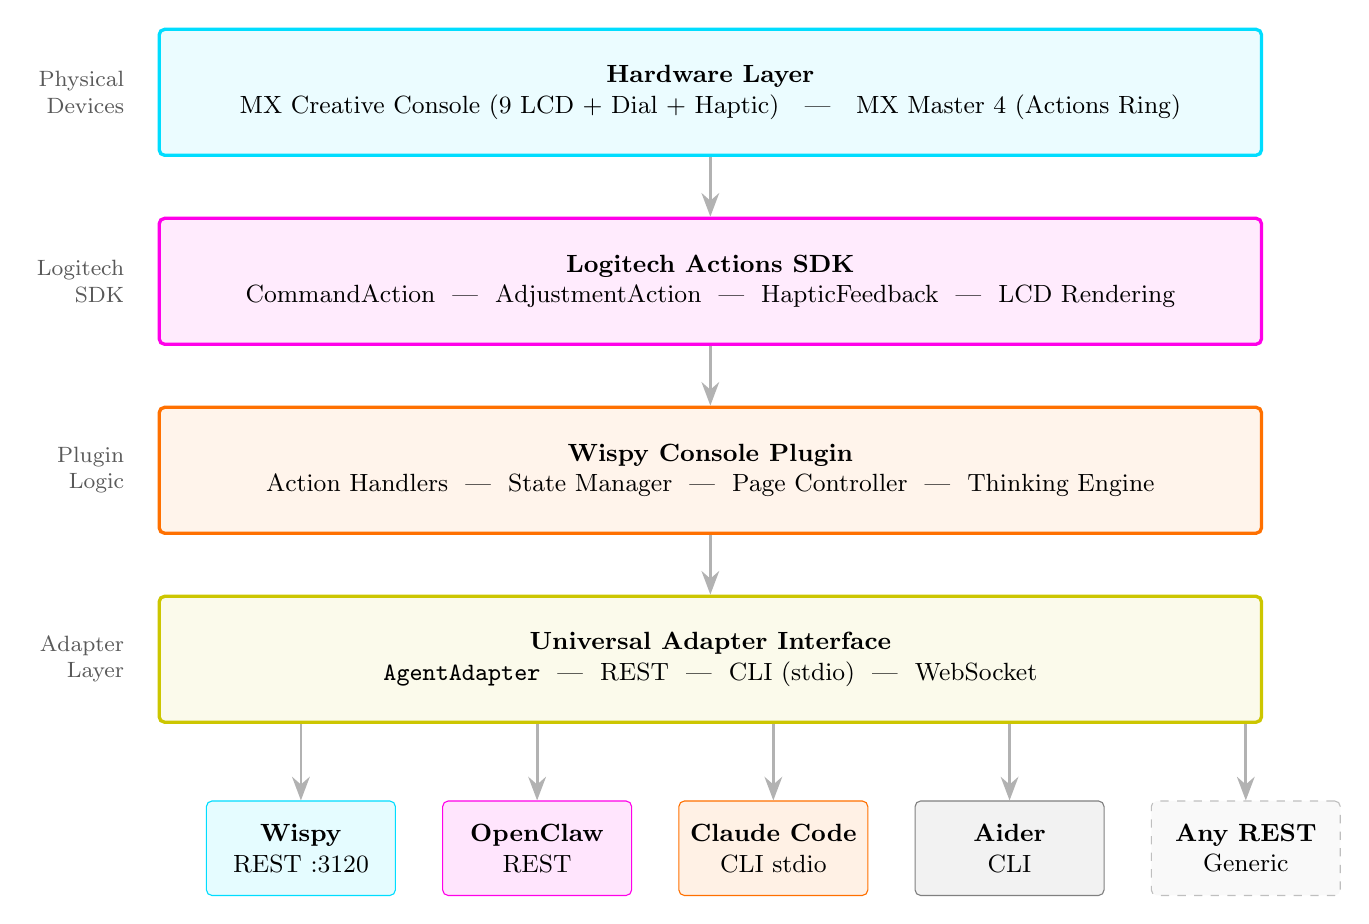
\begin{tikzpicture}[
  layer/.style={
    draw=#1, fill=#1!8, line width=1.2pt,
    minimum width=14cm, minimum height=1.6cm,
    rounded corners=2pt, align=center, font=\small
  },
  connector/.style={
    -{Stealth[length=3mm]}, line width=1pt, color=gray!60
  },
  label/.style={
    font=\footnotesize\color{gray!70!black}, align=right
  }
]

% Hardware Layer
\node[layer=wispycyan] (hw) at (0, 0) {
  \textbf{Hardware Layer}\\
  MX Creative Console (9 LCD + Dial + Haptic) ~~|~~ MX Master 4 (Actions Ring)
};
\node[label, left=3mm of hw.west, anchor=east] {Physical\\Devices};

% Actions SDK Layer
\node[layer=wispymagenta] (sdk) at (0, -2.4) {
  \textbf{Logitech Actions SDK}\\
  CommandAction ~|~ AdjustmentAction ~|~ HapticFeedback ~|~ LCD Rendering
};
\node[label, left=3mm of sdk.west, anchor=east] {Logitech\\SDK};

% Plugin Layer
\node[layer=wispyorange] (plugin) at (0, -4.8) {
  \textbf{Wispy Console Plugin}\\
  Action Handlers ~|~ State Manager ~|~ Page Controller ~|~ Thinking Engine
};
\node[label, left=3mm of plugin.west, anchor=east] {Plugin\\Logic};

% Adapter Layer
\node[layer=wispyyellow!80!black] (adapter) at (0, -7.2) {
  \textbf{Universal Adapter Interface}\\
  \texttt{AgentAdapter} ~|~ REST ~|~ CLI (stdio) ~|~ WebSocket
};
\node[label, left=3mm of adapter.west, anchor=east] {Adapter\\Layer};

% Agent boxes at bottom
\node[draw=wispycyan, fill=wispycyan!10, minimum width=2.4cm, minimum height=1.2cm, rounded corners=2pt, align=center, font=\small] (a1) at (-5.2, -9.6) {\textbf{Wispy}\\REST :3120};
\node[draw=wispymagenta, fill=wispymagenta!10, minimum width=2.4cm, minimum height=1.2cm, rounded corners=2pt, align=center, font=\small] (a2) at (-2.2, -9.6) {\textbf{OpenClaw}\\REST};
\node[draw=wispyorange, fill=wispyorange!10, minimum width=2.4cm, minimum height=1.2cm, rounded corners=2pt, align=center, font=\small] (a3) at (0.8, -9.6) {\textbf{Claude Code}\\CLI stdio};
\node[draw=gray, fill=gray!10, minimum width=2.4cm, minimum height=1.2cm, rounded corners=2pt, align=center, font=\small] (a4) at (3.8, -9.6) {\textbf{Aider}\\CLI};
\node[draw=gray!50, fill=gray!5, minimum width=2.4cm, minimum height=1.2cm, rounded corners=2pt, align=center, font=\small, dashed] (a5) at (6.8, -9.6) {\textbf{Any REST}\\Generic};

% Connections
\draw[connector] (hw) -- (sdk);
\draw[connector] (sdk) -- (plugin);
\draw[connector] (plugin) -- (adapter);
\draw[connector] (adapter.south -| a1) -- (a1);
\draw[connector] (adapter.south -| a2) -- (a2);
\draw[connector] (adapter.south -| a3) -- (a3);
\draw[connector] (adapter.south -| a4) -- (a4);
\draw[connector] (adapter.south -| a5) -- (a5);

\end{tikzpicture}
\end{center}

\subsection{Agent Adapter Interface}

The universal adapter interface defines the contract that any AI agent must implement to work with Wispy Console. The interface is intentionally minimal, focusing on the core interactions that physical hardware enables.

\vspace{3mm}

\begin{lstlisting}[language=Java, caption={AgentAdapter Interface (TypeScript)}]
interface AgentAdapter {
  /** Send a message or command to the agent */
  send(message: string, context?: AgentContext): Promise<AgentResponse>;

  /** Approve a pending action */
  approve(actionId: string): Promise<void>;

  /** Reject a pending action with optional feedback */
  reject(actionId: string, reason?: string): Promise<void>;

  /** Get current agent status and pending actions */
  getStatus(): Promise<AgentStatus>;

  /** Switch to a different agent or agent mode */
  switchAgent(agentId: string): Promise<void>;

  /** Set the thinking depth (0-100) */
  setThinkingDepth(level: number): Promise<void>;

  /** Get available tools for the current agent */
  getTools(): Promise<AgentTool[]>;

  /** Send voice input (audio buffer) to the agent */
  sendVoice(audio: Buffer, format: AudioFormat): Promise<AgentResponse>;
}

interface AgentStatus {
  state: 'idle' | 'thinking' | 'acting' | 'waiting' | 'error';
  pendingActions: PendingAction[];
  activeTools: string[];
  thinkingDepth: number;
  sessionDuration: number;
  tokensUsed: number;
}

interface PendingAction {
  id: string;
  type: 'file_write' | 'shell_exec' | 'api_call' | 'destructive';
  summary: string;
  risk: 'low' | 'medium' | 'high' | 'critical';
  timestamp: number;
}
\end{lstlisting}

\subsection{Supported Agents}

\begin{center}
\begin{tabularx}{\textwidth}{L{2.8cm} C{2.5cm} C{2cm} Y}
\toprule
\textbf{Agent} & \textbf{Protocol} & \textbf{Tools} & \textbf{Status} \\
\midrule
\rowcolor{wispylight}
Wispy & REST :3120 & 32+ & Reference implementation. Full adapter with all features. \\
OpenClaw & REST & Browser automation & Adapter ready. Browser-focused AI agent. \\
\rowcolor{wispylight}
Claude Code & CLI (stdio) & File, shell, search & Planned. CLI adapter for Anthropic's coding agent. \\
Aider & CLI & File, git & Planned. CLI adapter for AI pair programming. \\
\rowcolor{wispylight}
Any REST Agent & Generic REST & Variable & Generic adapter for any agent exposing a REST API. \\
\bottomrule
\end{tabularx}
\end{center}

\subsection{REST API Endpoints}

The plugin exposes a local REST API that adapters use to communicate with the hardware layer. This enables agents running in any environment (local process, Docker container, remote server) to interact with the physical console.

\vspace{3mm}

\begin{center}
\begin{tabularx}{\textwidth}{C{1.5cm} L{3.8cm} Y}
\toprule
\textbf{Method} & \textbf{Endpoint} & \textbf{Description} \\
\midrule
\rowcolor{wispylight}
POST & \texttt{/api/chat} & Send a message or command to the active agent \\
POST & \texttt{/api/agent/switch} & Switch the active agent by ID \\
\rowcolor{wispylight}
POST & \texttt{/api/approve} & Approve a pending action by action ID \\
POST & \texttt{/api/reject} & Reject a pending action with optional reason \\
\rowcolor{wispylight}
PUT & \texttt{/api/thinking} & Set thinking depth (0--100) \\
GET & \texttt{/api/status} & Get current agent status, pending actions, session info \\
\rowcolor{wispylight}
POST & \texttt{/api/voice} & Send voice audio buffer for speech-to-command \\
GET & \texttt{/api/tools} & List available tools for the active agent \\
\bottomrule
\end{tabularx}
\end{center}

\newpage

% ============================================================
% SECTION 5: EVIDENCE-BASED PROBLEM SOLVING
% ============================================================
\section{Evidence-Based Problem Solving}

Every design decision in Wispy Console is grounded in documented developer pain points. The following table maps each identified problem to its evidence source and the specific hardware solution.

\begin{hackathonbox}[title={\faClipboardCheck~Problem-Evidence-Solution Matrix}, breakable]

\begin{center}
\begin{tabularx}{\textwidth}{L{3cm} L{3.2cm} Y}
\toprule
\textbf{Problem} & \textbf{Evidence} & \textbf{Solution} \\
\midrule
\rowcolor{wispyyellowlight}
Permission Fatigue & GitHub \#2560, \#11380 (30+ upvotes, hundreds of comments) & \textbf{Physical Approve/Reject buttons.} Dedicated LCD buttons for approve and reject that require zero context switching. Thumb press replaces full-screen interrupt. \\

The YOLO Trap (Binary) & Hacker News discussion threads & \textbf{Thinking Dial with graduated control.} Continuous 0--100 dial replaces binary on/off. Four named zones (Flash, Standard, Deep Think, Marathon) provide intuitive reference points. \\

\rowcolor{wispyyellowlight}
Catastrophic YOLO & GitHub \#12637 (\texttt{rm -rf \textasciitilde/} incident) & \textbf{Physical danger zone on dial.} Marathon zone (81--100) provides haptic resistance and distinct feedback. Impossible to accidentally enter maximum autonomy. Press-to-reset returns to Standard. \\

Context Switching & Hacker News (@PetahNZ, @ak217) & \textbf{Dedicated hardware with haptic notifications.} Agent state communicated through vibration patterns. No need to switch windows. Status visible on LCD buttons at a glance. \\

\rowcolor{wispyyellowlight}
Multi-Agent Management & GitHub \#15898 (@midlifedad, 12 instances) & \textbf{Actions Ring agent switcher.} MX Master 4 ring provides instant agent switching. Context-aware auto-mapping reduces cognitive load from 12 terminals to one physical dial. \\

Accessibility Barriers & CHI 2025 Conference research & \textbf{Haptic + Voice + Physical buttons.} Non-visual state communication via 6 haptic patterns. Voice input via dedicated button. Large tactile targets for motor-impaired developers. \\

\rowcolor{wispyyellowlight}
Trust Crisis & Stack Overflow 2025 Survey (66\% correcting, 29\% trust) & \textbf{Graduated autonomy dial.} Thinking depth control lets developers trade speed for correctness. Higher depth activates deeper reasoning, chain-of-thought, and stricter review. Visible physical position provides trust transparency. \\

\bottomrule
\end{tabularx}
\end{center}

\vspace{3mm}

The critical insight is that these problems are fundamentally \textbf{interface problems}, not intelligence problems. AI agents are capable enough; the bottleneck is the human-agent interaction layer. Software-only solutions (chat UIs, terminal interfaces, IDE sidebars) all share the same constraint: they compete for the developer's visual attention on a single screen. Physical hardware operates on a separate sensory channel, enabling parallel awareness without context switching.

\end{hackathonbox}

\newpage

% ============================================================
% SECTION 6: IMPLEMENTATION
% ============================================================
\section{Implementation}

\subsection{Plugin Layer}

The plugin is built in TypeScript using the Logitech Actions SDK. Each physical interaction maps to an SDK action type that handles input, state management, and hardware feedback.

\vspace{3mm}

\begin{center}
\begin{tabularx}{\textwidth}{L{2.8cm} C{2.2cm} C{3cm} Y}
\toprule
\textbf{Action} & \textbf{SDK Type} & \textbf{Hardware} & \textbf{Function} \\
\midrule
\rowcolor{wispylight}
Code & CommandAction & LCD Button 1 & Send coding task to active agent \\
Research & CommandAction & LCD Button 2 & Initiate web research query \\
\rowcolor{wispylight}
Deploy & CommandAction & LCD Button 3 & Trigger deployment workflow \\
Approve & CommandAction & LCD Button 4 & Approve pending agent action \\
\rowcolor{wispylight}
Reject & CommandAction & LCD Button 5 & Reject pending action with reason \\
Voice & CommandAction & LCD Button 6 & Activate voice input for commands \\
\rowcolor{wispylight}
Status & CommandAction & LCD Button 7 & Display agent status summary \\
Quick & CommandAction & LCD Button 8 & Execute quick action shortcut \\
\rowcolor{wispylight}
Thinking Depth & AdjustmentAction & Dial (rotate) & Set thinking depth 0--100 \\
\bottomrule
\end{tabularx}
\end{center}

\vspace{3mm}

The plugin maintains a local state machine that tracks:

\begin{itemize}[leftmargin=5mm, itemsep=1mm]
  \item Current page (1--15) and active button configuration
  \item Active agent ID and connection status
  \item Thinking depth value and zone
  \item Queue of pending actions awaiting approval
  \item Session metrics (duration, tokens, actions approved/rejected)
\end{itemize}

\vspace{3mm}

LCD rendering updates at 200ms intervals during active agent operations, providing near-real-time visual feedback on each button's state.

\subsection{AI Engine: Wispy v1.4.1}

The reference AI engine is \textbf{Wispy v1.4.1}, published on npm as \texttt{wispy-ai}. Wispy serves as both the primary agent and the demonstration of the adapter interface's capabilities.

\vspace{3mm}

\begin{center}
\begin{tabularx}{\textwidth}{L{4cm} Y}
\toprule
\textbf{Feature} & \textbf{Details} \\
\midrule
\rowcolor{wispylight}
AI Model & Google Gemini 2.5 Pro (primary), Gemini 2.5 Flash (fast mode) \\
Tool Count & 32+ built-in tools (file, shell, git, web, memory, wallet) \\
\rowcolor{wispylight}
Marathon Mode & Multi-step autonomous planning and execution with checkpoints \\
Crypto Wallet & USDC payments via x402 protocol for paid API access \\
\rowcolor{wispylight}
Vector Memory & SQLite-backed vector store with embedding-based retrieval \\
Multi-Channel & REST API, Telegram, CLI REPL, MCP server \\
\rowcolor{wispylight}
Voice Support & Text-to-speech and speech-to-text via Gemini multimodal \\
Session Management & Persistent sessions with conversation history and context \\
\bottomrule
\end{tabularx}
\end{center}

\vspace{3mm}

Wispy exposes its REST API on port 3120 by default, which the Wispy Console plugin connects to via the \texttt{WispyAdapter} implementation of the \texttt{AgentAdapter} interface. All 32+ tools are automatically mapped to console pages, with the most frequently used tools on Page 1.

\subsection{Interactive Demo}

The submission includes an interactive Three.js + SVG demo that visualizes the complete Wispy Console experience in a browser. The demo features:

\begin{itemize}[leftmargin=5mm, itemsep=1mm]
  \item \textbf{3D Console Model}: Accurate representation of the MX Creative Console with clickable LCD buttons
  \item \textbf{Dial Interaction}: Draggable dial that demonstrates thinking depth zones with visual feedback
  \item \textbf{Auto-Demo Mode}: Automated sequence showing a complete agent workflow (task submission, thinking, approval, completion) with haptic visualization
  \item \textbf{Agent Switching}: Simulated Actions Ring interaction showing context-aware agent changes
  \item \textbf{Haptic Visualization}: Visual representation of each haptic pattern with animated waveforms
\end{itemize}

\vspace{3mm}

The demo serves as both a functional prototype and a visual explanation of the physical interactions that the plugin enables. It is accessible at the project's deployment URL and runs entirely client-side.

\newpage

% ============================================================
% SECTION 7: BUSINESS CASE
% ============================================================
\section{Business Case}

\begin{solutionbox}[title={\faTrophy~First-Mover Advantage}, breakable]

Wispy Console occupies an entirely uncontested market position: the intersection of physical hardware control and AI agent management. As of February 2026, this category does not exist.

\vspace{6mm}

\begin{center}
\begin{tikzpicture}[
  stat/.style={
    align=center, font=\bfseries
  }
]

% Stat 1
\node[stat] (s1) at (0, 0) {
  {\fontsize{36}{40}\selectfont\color{wispycyan} 40M+}\\[2mm]
  {\normalsize\color{wispyblack} MX Series Users\\Worldwide}
};

% Stat 2
\node[stat] (s2) at (5.5, 0) {
  {\fontsize{36}{40}\selectfont\color{wispymagenta} 73\%}\\[2mm]
  {\normalsize\color{wispyblack} Daily AI Tool\\Adoption Rate}
};

% Stat 3
\node[stat] (s3) at (11, 0) {
  {\fontsize{36}{40}\selectfont\color{wispyorange} 0}\\[2mm]
  {\normalsize\color{wispyblack} AI Plugins on\\Logitech Marketplace}
};

\end{tikzpicture}
\end{center}

\vspace{6mm}

The convergence of these three numbers defines the opportunity: a massive installed base of premium hardware users, the majority of whom use AI tools daily, with zero existing solutions connecting their hardware to their AI workflows.

\end{solutionbox}

\vspace{4mm}

\subsection{Pricing Model}

\begin{center}
\begin{tabularx}{\textwidth}{C{2.5cm} C{2.5cm} Y}
\toprule
\textbf{Tier} & \textbf{Price} & \textbf{Features} \\
\midrule
\rowcolor{wispylight}
\textbf{Free} & \$0/month & Core 9-button layout, single agent, 3 pages, basic haptic, community support \\
\textbf{Pro} & \$4.99/month & Voice commands, custom button layouts, multi-agent switching, Marathon mode integration, USDC wallet, 15 pages, all haptic patterns, priority support \\
\rowcolor{wispylight}
\textbf{Team} & \$9.99/month per seat & Shared console profiles, coordinated multi-agent workflows, team analytics dashboard, centralized configuration, admin controls \\
\bottomrule
\end{tabularx}
\end{center}

\vspace{3mm}

\subsection{Revenue Projections}

The pricing model targets three distinct segments:

\begin{itemize}[leftmargin=5mm, itemsep=2mm]
  \item \textbf{Free tier}: Maximizes adoption and marketplace visibility. Provides genuine value with core button functionality. Converts users through feature discovery (voice, multi-agent, Marathon mode are visible but locked).
  \item \textbf{Pro tier}: Targets individual developers who use AI agents daily. \$4.99/month is below the threshold for personal expense approval at most companies, reducing friction. Voice commands and multi-agent support are the primary conversion drivers.
  \item \textbf{Team tier}: Targets development teams using shared AI workflows. Shared profiles ensure consistent agent configurations across team members. Coordinated agents enable pair-programming-style workflows where multiple developers share agent state.
\end{itemize}

\vspace{3mm}

With 40M+ MX users and 73\% AI adoption, the addressable market is approximately 29M developers. Even a conservative 0.1\% conversion to the free tier (29,000 users) with 10\% Pro conversion yields meaningful recurring revenue.

\newpage

% ============================================================
% SECTION 8: CHALLENGES AND LESSONS
% ============================================================
\section{Challenges and Lessons}

\subsection{Challenges}

\begin{problembox}[title={\faExclamationCircle~Development Challenges}, breakable]

\begin{enumerate}[leftmargin=6mm, itemsep=3mm]
  \item \textbf{Alpha SDK Constraints}: The Logitech Actions SDK is in alpha, with documentation and APIs evolving rapidly. Several planned features (custom LCD rendering, advanced haptic sequences) required creative workarounds using available primitives. The SDK's TypeScript types occasionally lagged behind the actual runtime behavior, requiring empirical testing.

  \item \textbf{Mapping Abstract AI Concepts to Physical Hardware}: Translating concepts like ``thinking depth'' and ``agent trust level'' into physical dial positions required extensive user experience research. The initial prototype used discrete steps (4 positions), but user testing revealed that a continuous dial with named zones provided better intuitive control. Finding the right zone boundaries (0--20, 21--50, 51--80, 81--100) required iterating on the mapping between dial position and actual agent behavior changes.

  \item \textbf{Agent Normalization Complexity}: Different AI agents expose vastly different APIs, capabilities, and state models. Normalizing Wispy's 32-tool REST API, OpenClaw's browser automation commands, and a CLI agent's stdio interface into a single \texttt{AgentAdapter} interface required careful abstraction. The challenge was maintaining useful specificity (agents are genuinely different) while providing a uniform hardware interaction model.

  \item \textbf{15-Page UX Design}: Organizing up to 135 actions across 15 pages without overwhelming users required information architecture work. The solution of thematic page groups (core, tools, agents, projects, custom) emerged from card-sorting exercises and reflects how developers mentally categorize their AI interactions.

  \item \textbf{The YOLO Paradox}: Designing a physical control for ``how much should I trust the AI'' revealed a deeper design tension. Making the dial easy to turn toward high autonomy (for convenience) conflicts with making it hard to accidentally enable dangerous modes (for safety). The solution of haptic resistance zones, where the dial provides stronger feedback as it enters the Marathon range, resolves this tension through physical design rather than software constraints.
\end{enumerate}

\end{problembox}

\subsection{Lessons Learned}

\begin{wispybox}[title={\faLightbulb~Key Takeaways}, breakable]

\begin{enumerate}[leftmargin=6mm, itemsep=3mm]
  \item \textbf{The Actions SDK is well-designed for this use case.} Despite being in alpha, the SDK's action model (CommandAction for discrete inputs, AdjustmentAction for continuous inputs) maps naturally to AI agent interactions. The distinction between ``do this thing'' (button press) and ``adjust this parameter'' (dial turn) is exactly the distinction between agent commands and agent configuration.

  \item \textbf{Physical hardware adds an irreplaceable dimension.} No amount of software UI polish can replicate the ambient awareness that haptic feedback provides, or the zero-context-switch interaction of a physical button press. The console sits beside the keyboard, always visible, always accessible, operating on a sensory channel (touch) that software cannot reach. This is not a convenience improvement; it is a fundamentally different interaction modality.

  \item \textbf{The 15-page system is perfect for AI tool density.} Modern AI agents have 20--50+ tools, each with multiple modes and configurations. Traditional UIs collapse under this density, requiring nested menus, search interfaces, and keyboard shortcuts. The 15-page LCD grid provides flat, spatial organization where every action is at most two interactions away (page flip + button press). This scales to 135 actions without any nesting.

  \item \textbf{Accessibility is an untapped market.} The CHI 2025 research on AI accessibility barriers reveals a significant underserved population. Developers with RSI, visual impairments, and motor disabilities are not a niche; they represent a meaningful fraction of the professional developer community. Physical hardware with haptic feedback, voice input, and large tactile buttons is not an accommodation added after the fact. It is a primary design advantage that benefits all users while being essential for some.

  \item \textbf{Trust is a physical property.} The most surprising lesson was that making trust ``physical'' (a dial position you can see and feel) fundamentally changes the developer's relationship with AI autonomy. When trust is a checkbox in a settings panel, it is forgotten. When trust is the current position of a dial on your desk, it is ambient and continuous. This suggests that the entire category of AI safety controls could benefit from physicalization.
\end{enumerate}

\end{wispybox}

\newpage

% ============================================================
% SECTION 9: ROADMAP
% ============================================================
\section{Roadmap}

\begin{hackathonbox}[title={\faRoad~Development Roadmap}, breakable]

\textbf{\color{wispycyan}\faCircle~Phase 1: Hackathon Submission (Current)}

\vspace{2mm}

\begin{itemize}[leftmargin=5mm, itemsep=1mm]
  \item Complete plugin architecture with Actions SDK integration
  \item Universal \texttt{AgentAdapter} interface and adapter layer
  \item Interactive Three.js + SVG demo with auto-demo mode
  \item Wispy adapter (full REST integration with 32+ tools)
  \item OpenClaw adapter (browser automation agent)
  \item 9-button default layout with Page 1 configuration
  \item Thinking depth dial with 4 named zones
  \item Haptic feedback integration with 6 patterns
  \item Technical whitepaper and documentation
\end{itemize}

\vspace{4mm}

\textbf{\color{wispymagenta}\faCircle~Phase 2: Post-SDK General Availability}

\vspace{2mm}

\begin{itemize}[leftmargin=5mm, itemsep=1mm]
  \item Full LCD rendering with agent status icons and live counters
  \item Dynamic button icons that reflect real-time agent state
  \item Custom icon packs for different agent types
  \item LCD animation support for thinking states and progress indicators
  \item Advanced haptic sequences combining multiple patterns
  \item Button press-and-hold actions for secondary functions
\end{itemize}

\vspace{4mm}

\textbf{\color{wispyorange}\faCircle~Phase 3: Agent Ecosystem Expansion}

\vspace{2mm}

\begin{itemize}[leftmargin=5mm, itemsep=1mm]
  \item Claude Code adapter (CLI stdio protocol)
  \item Aider adapter (CLI integration for AI pair programming)
  \item Continue.dev adapter (IDE-native AI coding)
  \item Cursor adapter (AI-first code editor)
  \item Generic REST adapter with configuration UI
  \item Agent discovery and auto-configuration
  \item Community adapter marketplace for third-party agents
\end{itemize}

\vspace{4mm}

\textbf{\color{wispyyellow!80!black}\faCircle~Phase 4: Team and Collaboration}

\vspace{2mm}

\begin{itemize}[leftmargin=5mm, itemsep=1mm]
  \item Shared console profiles (export/import configurations)
  \item Coordinated multi-agent workflows across team members
  \item Team analytics dashboard (usage patterns, approval rates, thinking depth distribution)
  \item Role-based access control for team configurations
  \item Centralized agent policy management (minimum thinking depth, prohibited actions)
  \item Integration with team communication tools (Slack, Discord notifications)
\end{itemize}

\vspace{4mm}

\textbf{\color{gray}\faCircle~Phase 5: Platform Distribution}

\vspace{2mm}

\begin{itemize}[leftmargin=5mm, itemsep=1mm]
  \item Logitech Marketplace distribution (first AI plugin category)
  \item MX Ink integration for VR/AR agent interaction
  \item Wispy Console SDK for third-party plugin developers
  \item Enterprise deployment and management tools
  \item Cross-platform support verification (Windows, macOS, Linux)
  \item Accessibility certification and compliance testing
\end{itemize}

\end{hackathonbox}

\newpage

% ============================================================
% SECTION 10: TEAM AND LINKS
% ============================================================
\section{Team and Links}

\subsection{Team}

\begin{center}
\begin{tikzpicture}[
  card/.style={
    draw=gray!30, fill=white, rounded corners=5pt, line width=0.5pt,
    minimum width=7cm, minimum height=3.5cm, align=left,
    inner sep=8mm
  }
]

% Brian
\node[card] (brian) at (0, 0) {
  \begin{minipage}{5.5cm}
    {\large\bfseries Brian Mwai}\\[3mm]
    {\small\color{gray!70!black} Full-Stack Developer \& AI Agent Researcher}\\[2mm]
    {\small Creator of Wispy, an autonomous AI agent platform. Builder of developer tools that bridge AI capabilities with human workflows. Based in Nairobi, Kenya.}\\[3mm]
    {\small\color{wispymagenta!80!black} \faGithub~brn-mwai ~~\faTwitter~@brn\_mwai}
  \end{minipage}
};

% Joy
\node[card] (joy) at (0, -4.5) {
  \begin{minipage}{5.5cm}
    {\large\bfseries Joy Chepkoech Lang'at}\\[3mm]
    {\small\color{gray!70!black} Software Engineer}\\[2mm]
    {\small Wispy contributor and software engineer focused on building reliable, accessible software systems. Based in Nairobi, Kenya.}\\[3mm]
    {\small\color{wispymagenta!80!black} \faGithub~JoyyCLangat}
  \end{minipage}
};

% Hausor Labs
\node[card, draw=wispycyan!50, fill=wispylight] (hausor) at (0, -9) {
  \begin{minipage}{5.5cm}
    {\large\bfseries Hausor Labs}\\[3mm]
    {\small\color{gray!70!black} Building Autonomous AI Tools for Developers}\\[2mm]
    {\small An independent lab focused on the intersection of AI agents, developer experience, and physical computing. Our mission is to make AI agents genuinely useful through better human-agent interfaces.}\\[3mm]
    {\small\color{wispymagenta!80!black} \faGlobe~hausorlabs.tech}
  \end{minipage}
};

\end{tikzpicture}
\end{center}

\subsection{Links}

\begin{center}
\begin{tabularx}{\textwidth}{L{3.5cm} Y}
\toprule
\textbf{Resource} & \textbf{URL} \\
\midrule
\rowcolor{wispylight}
npm Package & \url{https://www.npmjs.com/package/wispy-ai} \\
GitHub Repository & \url{https://github.com/brn-mwai/wispy} \\
\rowcolor{wispylight}
Website & \url{https://wispy.cc} \\
Platform & \url{https://app.wispy.cc} \\
\rowcolor{wispylight}
Documentation & \url{https://docs.wispy.cc} \\
X / Twitter & \url{https://x.com/brn_mwai} \\
\rowcolor{wispylight}
Hausor Labs & \url{https://hausorlabs.tech} \\
\bottomrule
\end{tabularx}
\end{center}

\vspace{8mm}

\begin{center}

\begin{tikzpicture}
  \fill[wispycyan] (0,0) rectangle (4,0.1);
  \fill[wispymagenta] (4.2,0) rectangle (8.2,0.1);
  \fill[wispyorange] (8.4,0) rectangle (12.4,0.1);
  \fill[wispyyellow] (12.6,0) rectangle (16.6,0.1);
\end{tikzpicture}
\end{center}

\vspace{4mm}

\begin{center}
{\small\color{gray!60!black} Wispy Console -- Technical Whitepaper v1.0 -- February 2026}\\[2mm]
{\small\color{gray!60!black} Built for DevStudio 2026 by Logitech}\\[2mm]
{\small\color{gray!60!black} \textcopyright~2026 Hausor Labs. All rights reserved.}
\end{center}

\end{document}
